\chapter{Anexos}
	\noident Este apartado está dedicado para la consulta de archivos que se emplean dentro del documento. 
	\section{Apartado A: Diseños de Pantallas}
	
		\begin{figure}[hbt!]
			\centering
			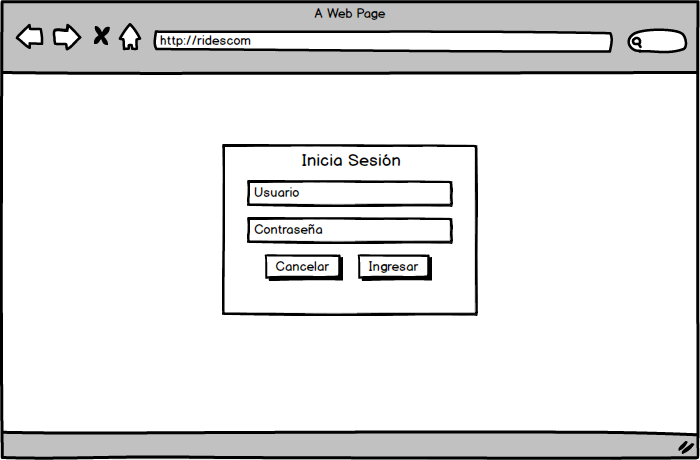
\includegraphics[width=10cm, height=6cm]{Imagenes/Nuevos/P1_LoginJFD_coord}
			\caption{Inicio sesión para el JFD y el coordinador de U.A.}
			\label{inicioJFDycoord}
		\end{figure}
		\pagebreak
		
		\begin{figure}[hbt!]
			\centering
			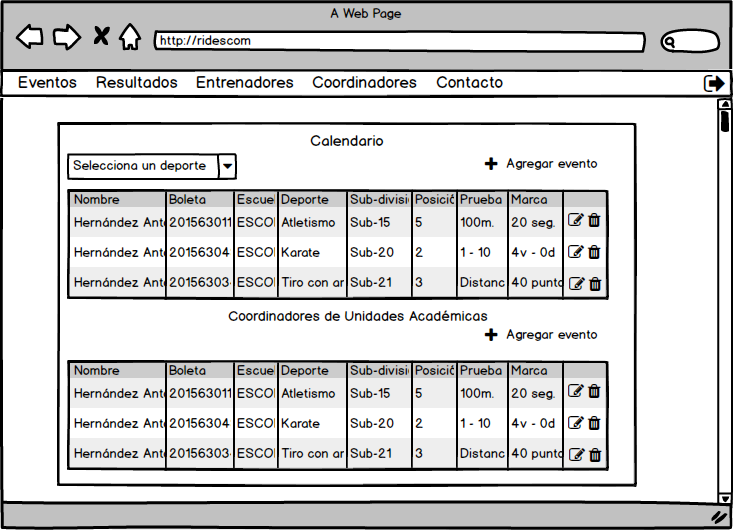
\includegraphics[width=10cm, height=6cm]{Imagenes/Nuevos/P2_Inicio_JefeFD}
			\caption{Página principal para el Jefe de Fomento Deportivo}
			\label{principalJFD}
		\end{figure}
	
		\begin{figure} [hbt!]
			\centering
			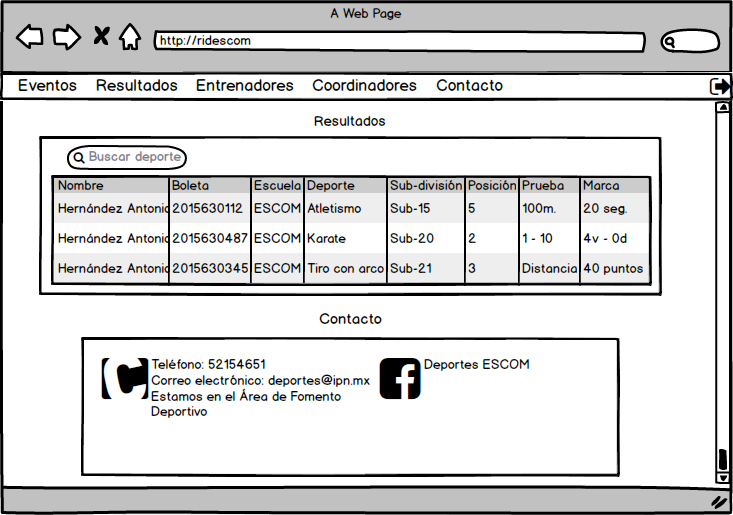
\includegraphics[width=10cm, height=6cm]{Imagenes/Nuevos/P3_Inicio_JefeFD1}
			\caption{Página principal para el Jefe de Fomento (Continuación).}
			\label{principalJFD1}
		\end{figure}
	
		\begin{figure} [hbt!]
			\centering
			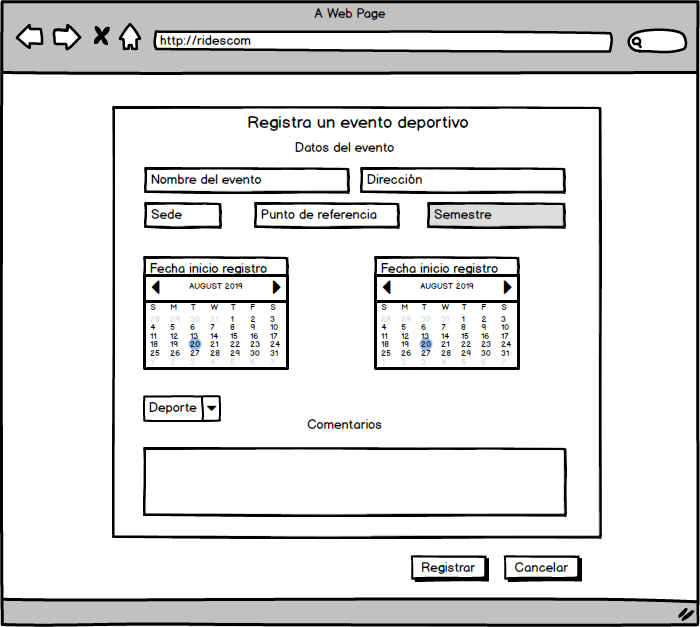
\includegraphics[width=10cm, height=6cm]{Imagenes/Nuevos/P4_Crear_evento_deportivo}
			\caption{Vista para dar de alta un evento deportivo (Jefe de Fomento Deportivo).}
			\label{creaevento}
		\end{figure}
		
		\pagebreak	
		
		\begin{figure} [hbt!]
			\centering
			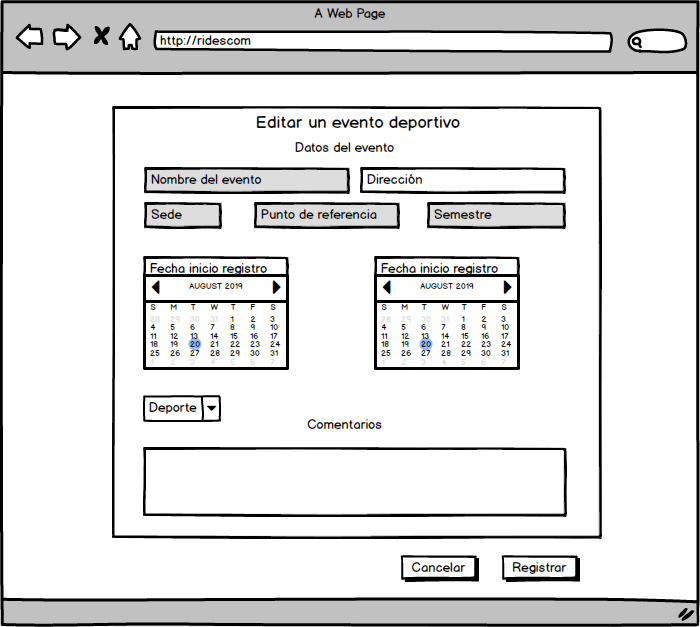
\includegraphics[width=10cm, height=6cm]{Imagenes/Nuevos/P5_Editar_evento_deportivo}
			\caption{Vista para editar datos de un evento ya registrado. (Jefe de FOmento Deportivo).}
			\label{editarevento}
		\end{figure}
	
		\begin{figure} [hbt!]
			\centering
			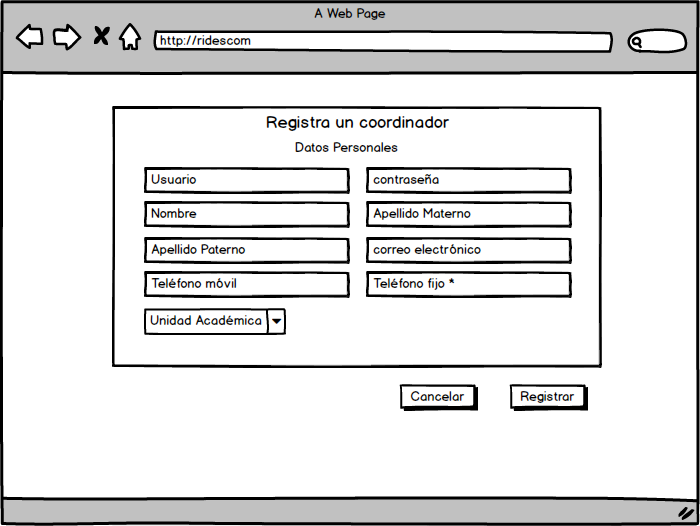
\includegraphics[width=10cm, height=6cm]{Imagenes/Nuevos/P6_Registro_coordinador}
			\caption{Vista para registrar un coordinador de unidad académica. (Jefe de Fomento Deportivo).}
			\label{registrarcoord}
		\end{figure}
		
		\begin{figure} [hbt!]
			\centering
			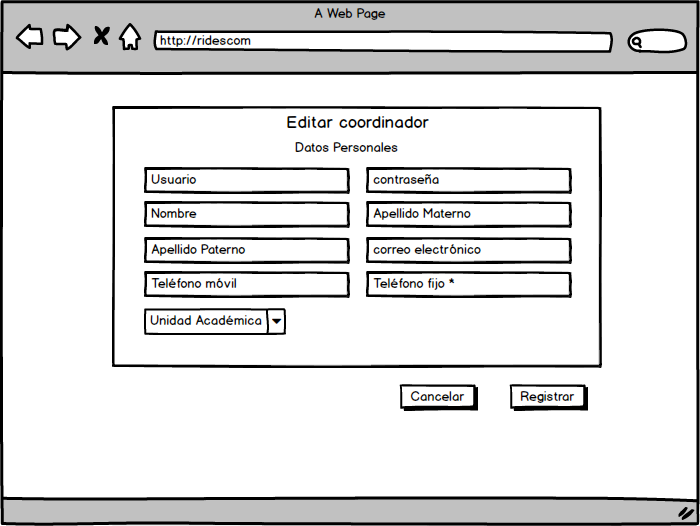
\includegraphics[width=10cm, height=6cm]{Imagenes/Nuevos/P7_Editar_coordinador}
			\caption{Vista para editar datos de un coordinador previamente registrado. (Jefe de Fomento Deportivo).}
			\label{editarcoord}
		\end{figure}
\pagebreak

		\begin{figure} [hbt!]
			\centering
			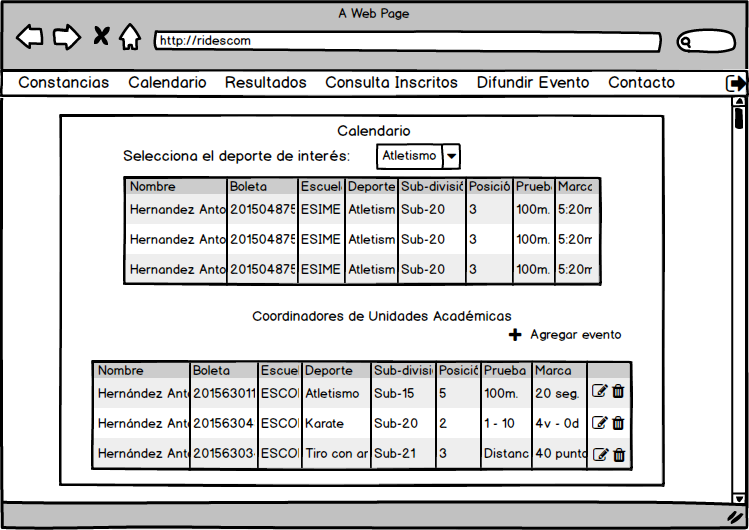
\includegraphics[width=10cm, height=6cm]{Imagenes/Nuevos/P8_Inicio_CoordUA}
			\caption{Vista principal para el coordinador de una Unidad Académica.}
			\label{principalcoord}
		\end{figure}
	
		\begin{figure} [hbt!]
			\centering
			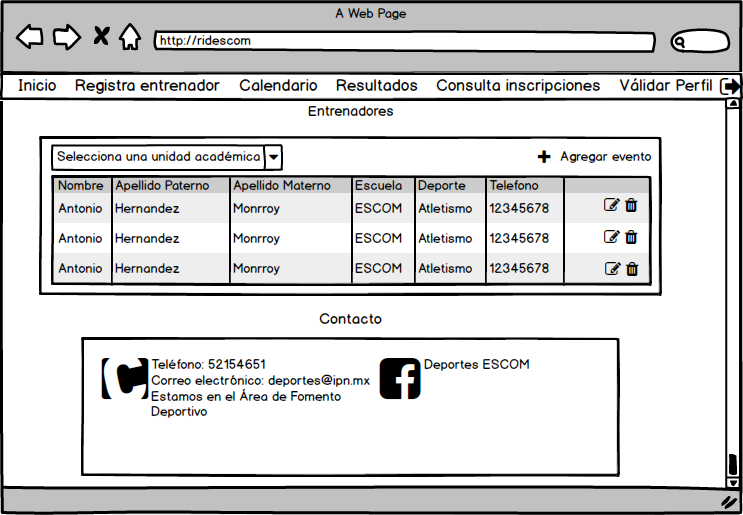
\includegraphics[width=10cm, height=6cm]{Imagenes/Nuevos/P9_Inicio_CoordUA1}
			\caption{Vista principal para el coordinador de una Unidad Académica (Continuación).}
			\label{principalcoord1}
		\end{figure}
	\pagebreak
		
		\begin{figure} [hbt!]
			\centering
			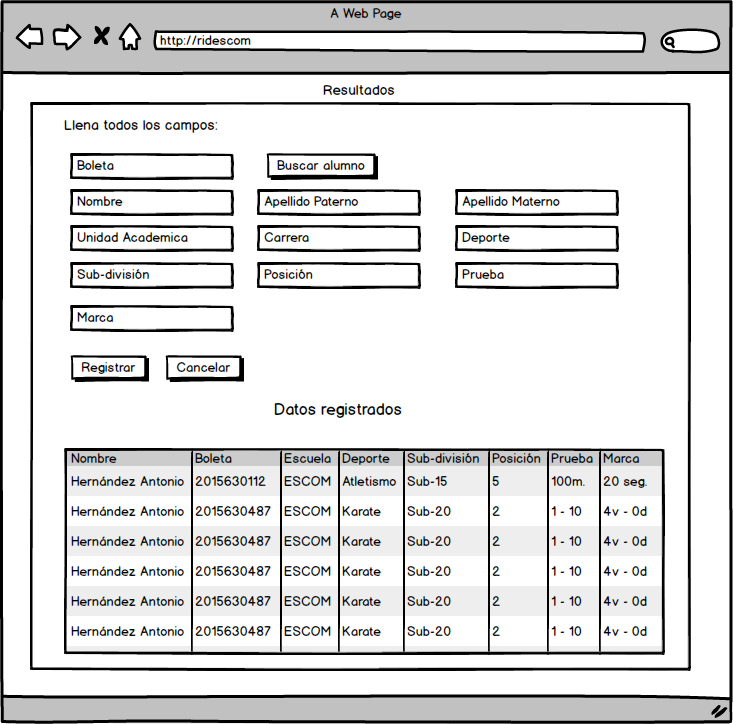
\includegraphics[width=10cm, height=7cm]{Imagenes/Nuevos/P10_Ingresa_resultados}
			\caption{Vista para ingresar los resultados obtenidos por los participantes (Coordinador de Unidad Académica).}
			\label{ingresaresultados}
		\end{figure}
		
		\begin{figure} [hbt!]
			\centering
			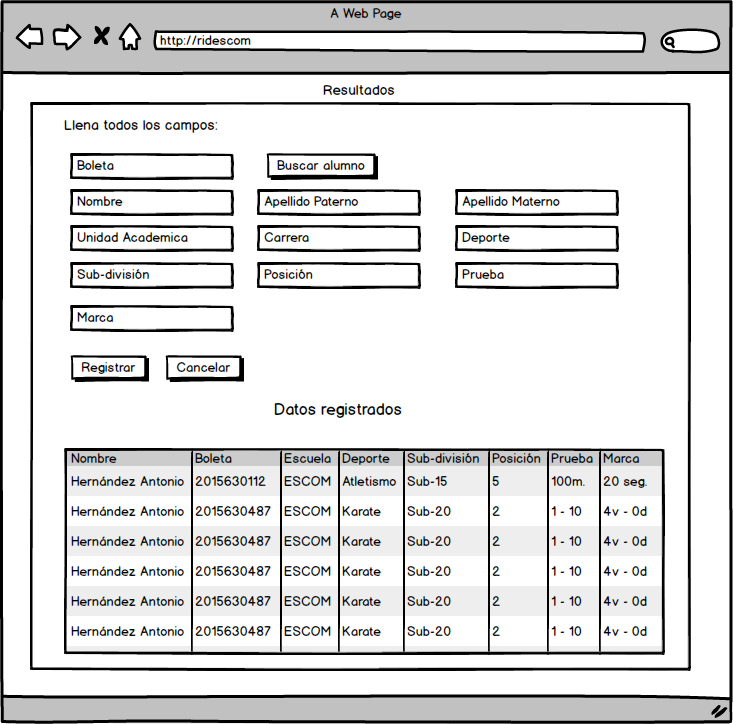
\includegraphics[width=10cm, height=7cm]{Imagenes/Nuevos/P11_Editar_resultados}
			\caption{Vista para editar los resultados de los participantes (Coordinador de Unidad Académica).}
			\label{editaresultados}
		\end{figure}
	\pagebreak
		
		\begin{figure} [hbt!]
			\centering
			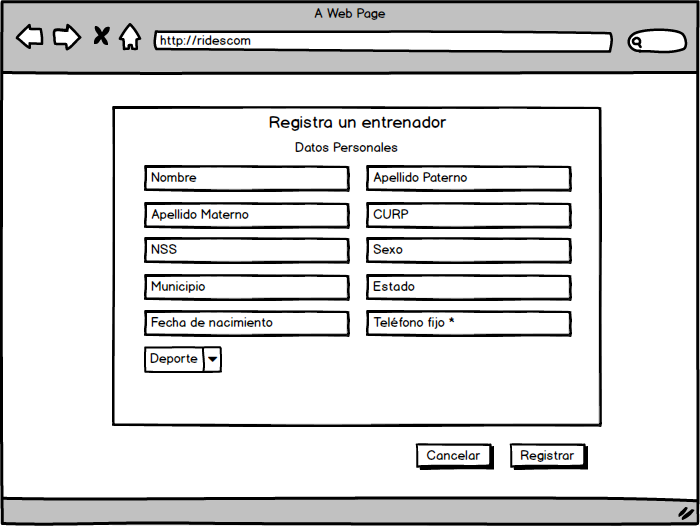
\includegraphics[width=10cm, height=6cm]{Imagenes/Nuevos/P12_Registro_entrenador}
			\caption{Vista para registrar a un entrenador (Coordinador de Unidad Académica).}
			\label{registroentrenador}
		\end{figure}
		
		\begin{figure} [hbt!]
			\centering
			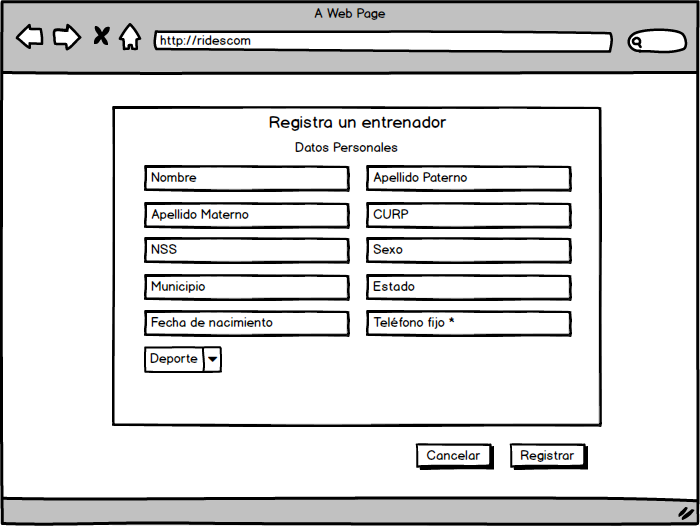
\includegraphics[width=10cm, height=6cm]{Imagenes/Nuevos/P13_Editar_entrenador}
			\caption{Vista para editar los datos del entrenador (Coordinador de Unidad Académica).}
			\label{editarentrenador}
		\end{figure}
		
		\begin{figure} [hbt!]
			\centering
			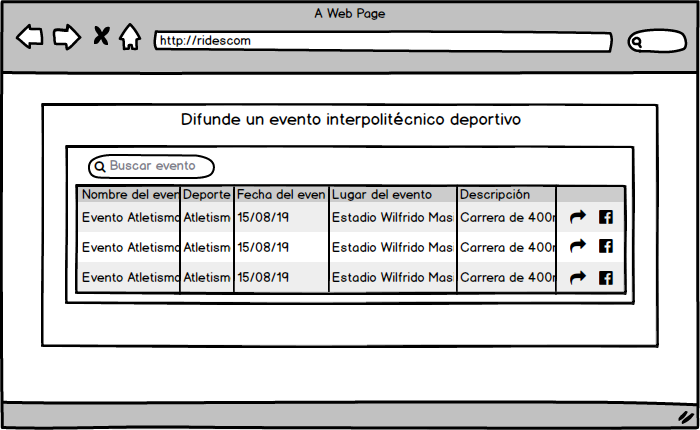
\includegraphics[width=10cm, height=6cm]{Imagenes/Nuevos/P14_Difundir_evento}
			\caption{Vista para difundir un evento interpolitécnico deportivo (Coordinador de Unidad Académica).}
			\label{difundirevento}
		\end{figure}
	\pagebreak
		\begin{figure} [hbt!]
			\centering
			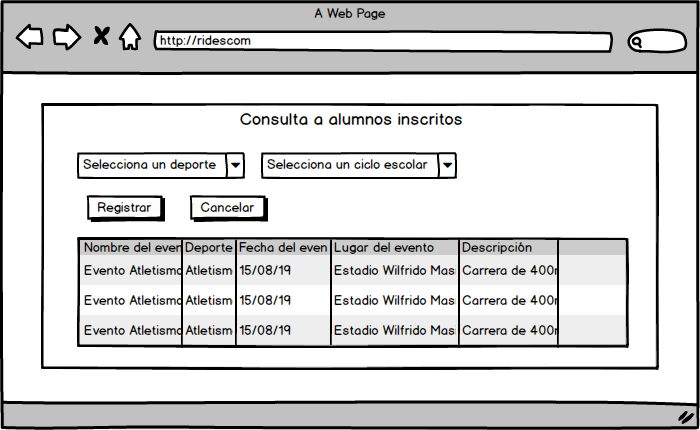
\includegraphics[width=10cm, height=6cm]{Imagenes/Nuevos/P15_Consulta_alumnos_inscritos}
			\caption{Vista para consultar los alumnos que se han inscrito a un evento (Coordinador de Unidad Académica).}
			\label{consultaalumnosinscritos}
		\end{figure}
	
		\begin{figure} [hbt!]
			\centering
			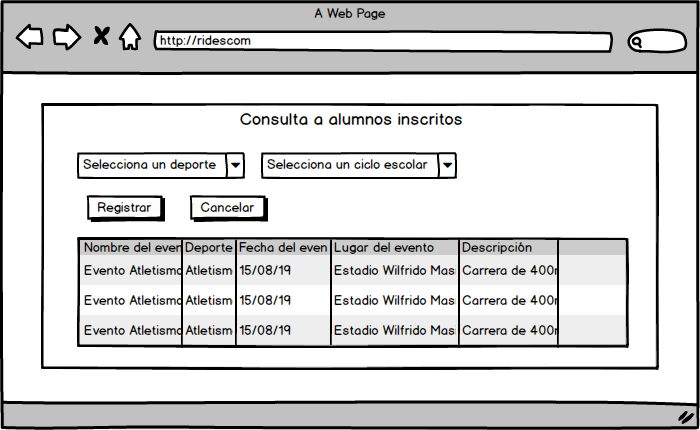
\includegraphics[width=10cm, height=6cm]{Imagenes/Nuevos/P16_Consulta_para_expedir_constancias}
			\caption{Vista para consultar participación de alumnos (Coordinador).}
			\label{consultaparaexpedirconstancias}
		\end{figure}
		
		\begin{figure} [hbt!]
			\centering
			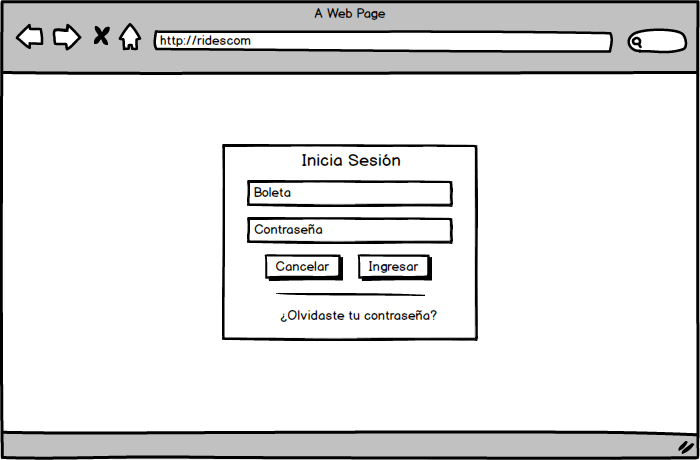
\includegraphics[width=10cm, height=6cm]{Imagenes/Nuevos/P17_Login_alumno}
			\caption{Vista Inicio de Sesión para el alumno.}
			\label{loginalumno}
		\end{figure}
		
	\pagebreak
		\begin{figure} [hbt!]
			\centering
			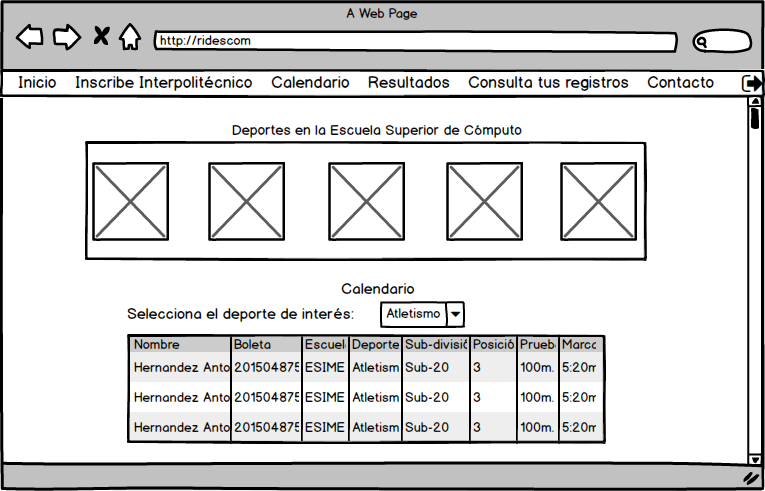
\includegraphics[width=10cm, height=6cm]{Imagenes/Nuevos/P18_Inicio_paticipante}
			\caption{Vista principal del alumno.}
			\label{principalalum}
		\end{figure}
		
		\begin{figure} [hbt!]
			\centering
			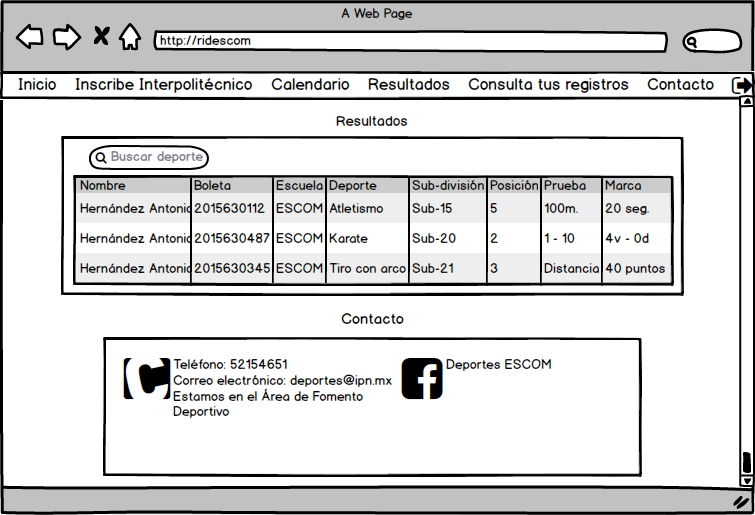
\includegraphics[width=10cm, height=6cm]{Imagenes/Nuevos/P19_Inicio_paticipante1}
			\caption{Vista principal del alumno (Continuación).}
			\label{principalalum1}
		\end{figure}
	
		\begin{figure} [hbt!]
			\centering
			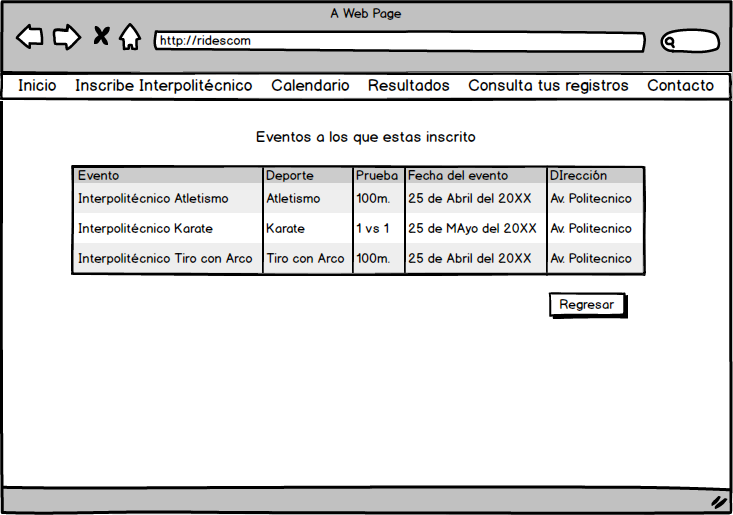
\includegraphics[width=10cm, height=6cm]{Imagenes/Nuevos/P20_Consulta_Inscripciones}
			\caption{Vista para consultar los eventos a los que se a registrado el alumno (Alumno).}
			\label{consultainscripcion}
		\end{figure}
	\pagebreak
		
		\begin{figure} [hbt!]
			\centering
			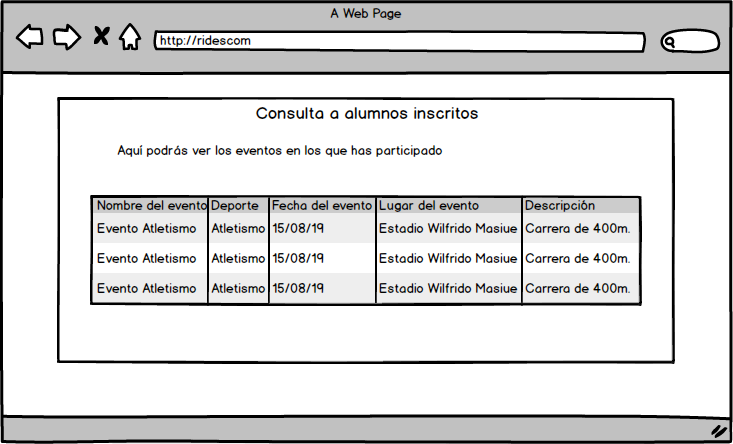
\includegraphics[width=10cm, height=6cm]{Imagenes/Nuevos/P21_Historial}
			\caption{Vista para que el alumno pueda visualizar todos los eventos en los que ha participado.}
			\label{historial}
		\end{figure}
		
		

	\section{Apartado B: Diagrama de Procesos}	
		
		\begin{figure}[hbt!]
			\centering
			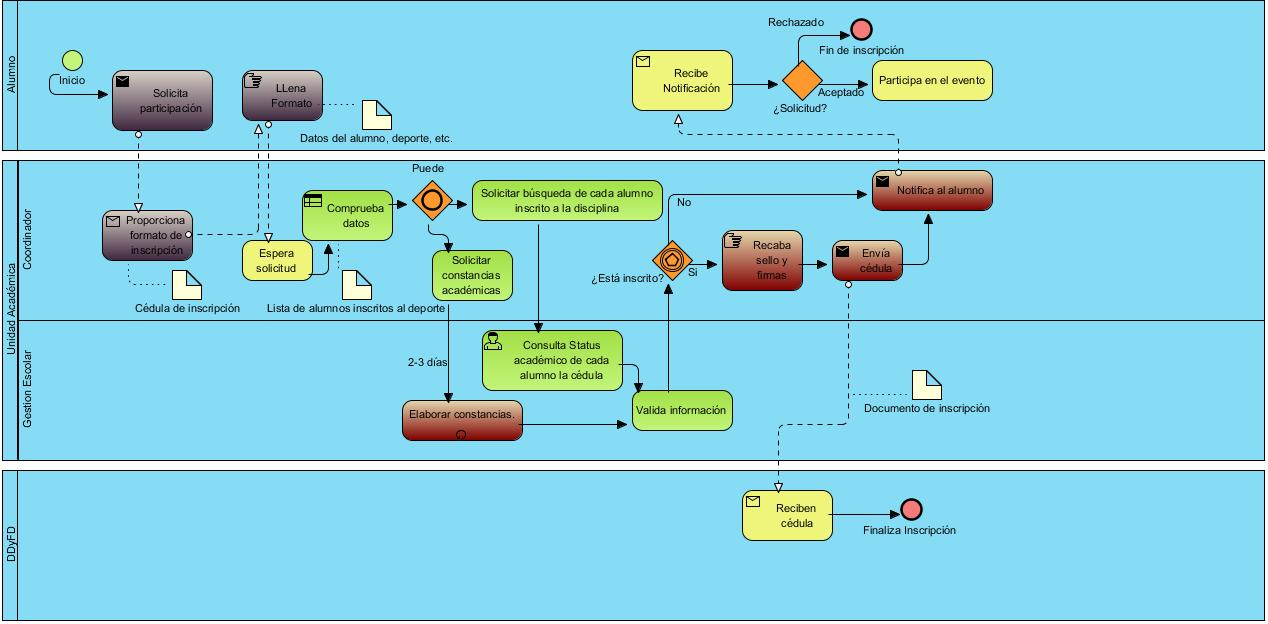
\includegraphics[width=16cm, height=8cm]{Imagenes/Disenos/ProcesoInscripcionActual.jpg}
			\caption{Proceso actual para la inscripcion a un evento interpolitécnico deportivo.}
			\label{ProcesoInscripcionActual}
		\end{figure}
	
		\begin{figure}[hbt!]
			\centering
			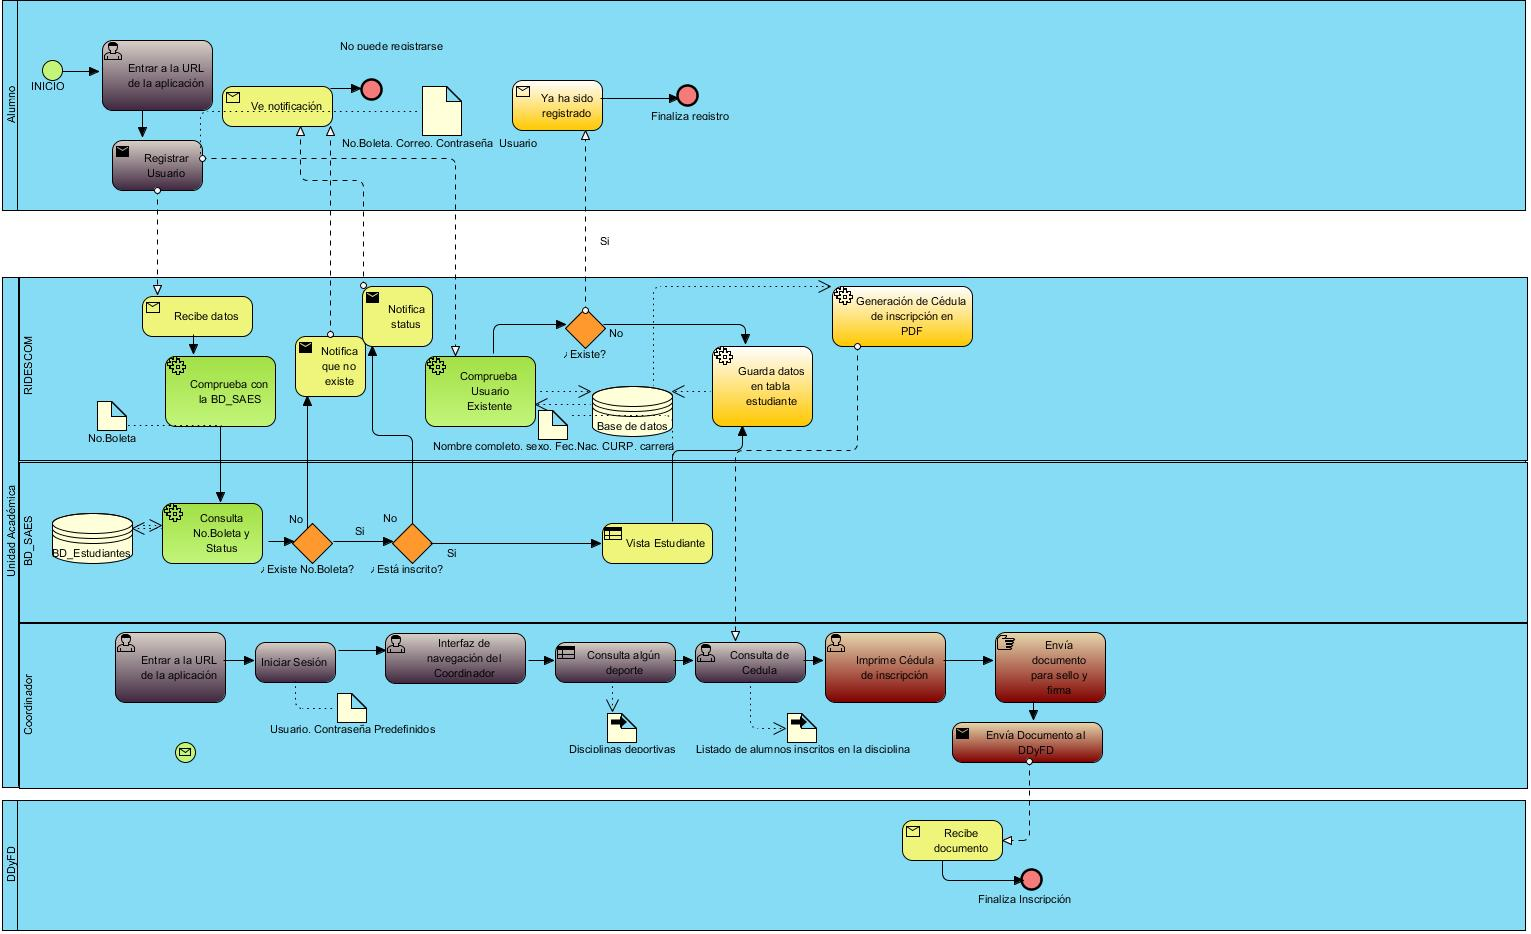
\includegraphics[width=16cm, height=8cm]{Imagenes/Disenos/ProcesoInscripcionPropuesto.jpg}
			\caption{Proceso propuesto para la inscripcion a un evento interpolitécnico deportivo.}
			\label{ProcesoInscripcionPropuesto}
		\end{figure}
	
		
	
	\pagebreak
	
	\section{Apartado C: Diagramas de Casos de Uso}
		\begin{figure}[hbt!]
			\centering
			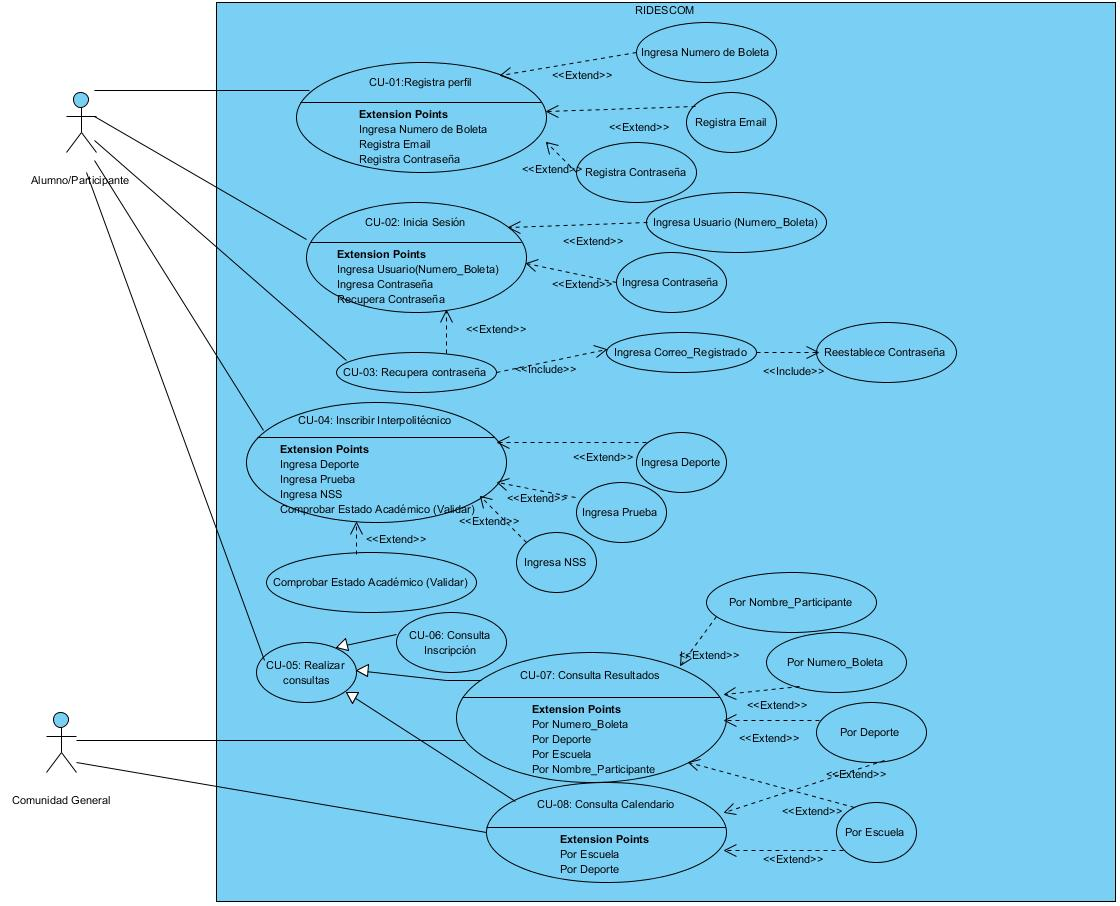
\includegraphics[width=16cm, height=8cm]{Imagenes/Disenos/DiagramasCU/Alumno.jpg}
			\caption{Diagrama de procesos Inscripción actual para un evento interpolitécnico deportivo.}
			\label{Inscripcion}
		\end{figure}
		\begin{figure}[hbt!]
			\centering
			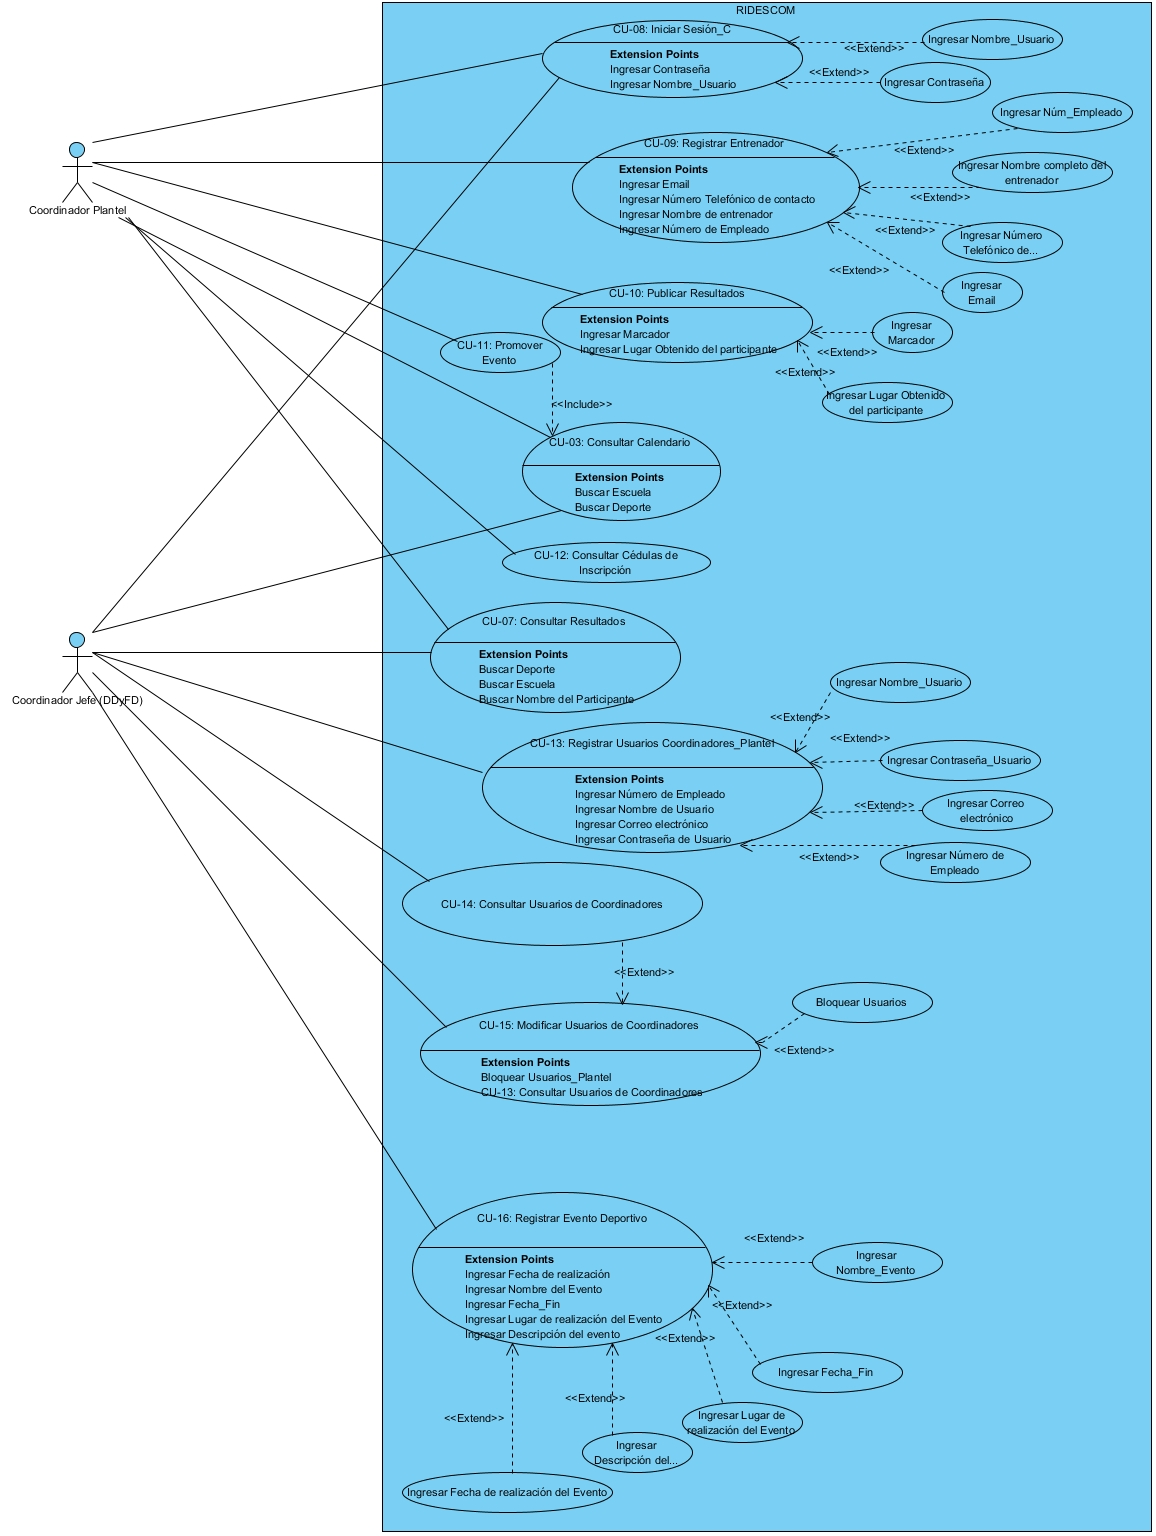
\includegraphics[width=16cm, height=12cm]{Imagenes/Disenos/DiagramasCU/CoordinadoresFinal.jpg}
			\caption{Diagrama de procesos Inscripción propuesto para un evento interpolitécnico deportivo.}
			\label{Inscripcion}
		\end{figure}
	\pagebreak

	\section{Apartado D: Casos de Uso}
		\label{CasosdeUso}
		\begin{UseCase}{CU1}{Iniciar Sesión Jefe de Fomento Deportivo}{
		\noindent Esta caso de uso servirá para que el Jefe de Fomento Deportivo pueda ingresar a la página web, poder identificar al usuario y así mostrar las vistas que tienen asginada. \\
    	Para poder iniciar sesión el actor deberá oprimir el botón \IUbutton{ Iniciar Sesión } ubicado en la pantalla \ref{inicioJFDycoord}. Ingresará su número de boleta, contraseña el cual usa para ingresar al SAES (Sistema de Administración Escolar), y el captcha, como se muestra en la pantalla... Si los datos que ingresa no coinciden se le mostrará un mensaje.
        Una vez que incie sesión se le mostrará la pantalla principal.
        \MSGref{MSG1}{Campos requeridos}.
        
	} \label{CU1_Iniciarsesion}
		\UCitem{Versión}{0.1}
		\UCitem{Autor}{Rosales González Carlos Andrés}
		\UCitem{Supervisa}{Mendoza García Bruno Alejandro}
		\UCitem{Actor}{Jefe de Fomento Deportivo}
		\UCitem{Propósito}{Tener control de las personas registradas.}
        \UCitem{Precondiciones}{
        \begin{itemize}
            \item Contar con una cuenta.
            \item Contar con la contraseña.
        \end{itemize}}
        \UCitem{Postcondiciones}{Se muestra la pantalla principal}
		\UCitem{Entradas}{
        \begin{itemize}
        	\item Usuario. 
        	\item Contraseña
        \end{itemize}}
		\UCitem{Origen}{Pantalla, Teclado}
		\UCitem{Salidas}{
		\begin{itemize}
		    \item Acceso a la página principal del Jefe de Fomento Deportivo
		\end{itemize}}
		\UCitem{Destino}{Pantalla}
		\UCitem{Errores}{
        	\begin{itemize}
        	    \item Los campos están vacíos.
            	\item Usuario y/o contraseña incorrecta.
            \end{itemize}
       }
		\UCitem{Observaciones}{}
		\end{UseCase}
	\newpage
	
    \begin{UCtrayectoria}{Principal}
    \UCpaso[\UCactor] Ingresa a la página RIDESCOM.
    \UCpaso Muestra la pantalla \IUref{}{Pantalla de Inicio de Sesión \ref{inicioJFDycoord}}.
    \UCpaso[\UCactor] Oprime el botón \IUbutton{ JFD o Coordinador } que esta en la \IUref{}{Pantalla de Inicio de Sesión \ref{inicioJFDycoord}}.
    \UCpaso Muestra la \IUref{}{Pantalla de Inicio de Sesión \ref{inicioJFDycoord}}
	\UCpaso[\UCactor] Introduce Usuario y contraseña. \label{CU1_regresar} 
    \UCpaso[\UCactor] Presiona el botón \IUbutton{ Ingresar }.
    \UCpaso Comprueba que los campos no estén vacíos. \Trayref{A}
    \UCpaso Obtiene los valores ingresados
    \UCpaso Válida campos. \Trayref{B}
    \UCpaso Muestra la \IUref{}{Pantalla principal del Jefe de Fomento Deportivo. \ref{principalJFD}}
    \end{UCtrayectoria}
    
    \begin{UCtrayectoriaA}{A}{Campo(s) vacios}
    	\UCpaso muestra mensaje “CamposNecesario".
    	\UCpaso Continua en el paso \ref{CU1_regresar} del \UCref{CU1}.
    \end{UCtrayectoriaA}

	\begin{UCtrayectoriaA}{B}{Boleta y/o contraseña erróneo}
		\UCpaso muestra mensaje “El usuario y/o contraseña que se ingresó son erróneos”. Mensaje .
   		\UCpaso Continua en el paso \ref{CU1_regresar} del \UCref{CU1}.
	\end{UCtrayectoriaA}

	



		\begin{UseCase}{CU1.1}{Inicio Sesión}{
		Servirá para que el alumno pueda ingresar a la aplicación y así poder inscribirse en algún evento de su interés o consultar los eventos a los que ya se ha registrado previamente. \\
        En caso de que el alumno ingrese una boleta la cual no a sido registrada, se mostrará un mensaje el cual le indique que la boleta que ingreso no existe. Mensaje . De igual manera, si la contraseña es diferente a la que se registro aparecerá un mensaje que le indique que la contraseña no coincide. Mensaje .
	}
		\UCitem{Versión}{0.1}
		\UCitem{Autor}{Rosales González Carlos Andrés}
		\UCitem{Supervisa}{Mendoza García Bruno Alejandro}
		\UCitem{Actor}{Alumno}
		\UCitem{Propósito}{Tener control de las personas registradas.}
        \UCitem{Precondiciones}{
        \begin{itemize}
            \item Haberse registrado
            \item Perfil valido por el coordinador
        \end{itemize}}
        \UCitem{Postcondiciones}{Ninguna}
		\UCitem{Entradas}{
        \begin{itemize}
        	\item Número de boleta 
        	\item Contraseña
        \end{itemize}}
		\UCitem{Origen}{Pantalla, Teclado}
		\UCitem{Salidas}{
		\begin{itemize}
		    \item Acceso a la página principal del alumno
		\end{itemize}}
		\UCitem{Destino}{Pantalla}
		\UCitem{Errores}{
        	\begin{itemize}
        	    \item Los campos están vacíos.
            	\item No existe la boleta. Mensaje .
            	\item Contraseña incorrecta. Mensaje .
            \end{itemize}
       }
		\UCitem{Observaciones}{}
		\end{UseCase}
    \begin{UCtrayectoria}{Principal}
    \UCpaso[\UCactor] Oprime el botón Iniciar Sesión en la pantalla.
    \UCpaso Muestra la pantalla.
	\UCpaso[\UCactor] Introduce Boleta y contraseña. 
    \UCpaso[\UCactor] Presiona el botón Ingresar.
    \UCpaso Comprueba que los campos no estén vacíos. \Trayref{A} \Trayref{B} \Trayref{C}
    \UCpaso Obtiene los valores ingresados
    \UCpaso Válida campos. 
    \UCpaso Muestra la pantalla .
    \end{UCtrayectoria}
    
	\begin{UCtrayectoriaA}{A}{No hay dato insertado en el campo solicitado}
		\UCpaso muestra mensaje “Error: Los campos están vacíos por favor asegúrese de poner lo que se pide”. Mensaje .
		\UCpaso Regresa al paso 3 de la Trayectoria Principal.
	\end{UCtrayectoriaA}
	
	\begin{UCtrayectoriaA}{B}{}
		\UCpaso muestra mensaje “No existe boleta ingresada”. Mensaje .
		\UCpaso Regresa al paso 2 de la trayectoria principal.
	\end{UCtrayectoriaA}
	
	\begin{UCtrayectoriaA}{C}{}
		\UCpaso muestra mensaje “Contraseña incorrecta”. Mensaje .
		\UCpaso Regresa al paso 2 de la trayectoria principal.
	\end{UCtrayectoriaA}
		\begin{UseCase}{CU3}{Inscribir a un evento interpolitécnico deportivo}{
		\noindent Este caso de uso permite que el actor alumno, pueda registrarse en el evento interpolitécnico deportivo de su interés. Deberá llenar un formulario donde se solicitan datos del alumno como: Grupo, NSS (Número de Seguro Social), correo electrónico, Delegación/Municipio, así como el seleccionar el deporte en el que desea participar.\\
        Para poder inscribirse, deberá primero validar su estatus académico (Inscrito/No inscrito), para ello debe ingresar su boleta, contraseña y el captcha como se muestra en la pantalla \IUref{p15InscripcionInterpolitecnico1}{Pantalla Inscribir interpolitécnico 1.}, da click en el botón \IUbutton { Verificar } si cumple con el requisito, continua el proceso, en caso contrario no podrá inscribirse en algun evento interpolitécnico deportivo.\\
        El siguiente paso es la verificación de datos como se muestra en la pantalla \IUref{p15InscripcionInterpolitecnico2}{Pantalla Inscribir interpolitécnico 2.}, si los datos son correctos da click en el botón \IUbutton{ Aceptar }\\
        Si los datos son correctos, da click en el botón \IUbutton{ Aceptar }, a continuación se muestra la pantalla \IUref{p15InscripcionInterpolitecnico3}{Pantalla Inscribir interpolitécnico 3.} donde llenará los datos corresponidentes al evento deportivo. Una vez que se llenen todos los campos, el alumno da click en el botón \IUbutton{ Inscribir }.\\ 
        Al final se mostrará un mensaje de confirmación de la inscripción.
	}
		\UCitem{Versión}{0.1}
		\UCitem{Autor}{Rosales González Carlos Andrés}
		\UCitem{Supervisa}{Mendoza García Bruno Alejandro}
		\UCitem{Actor}{Alumno}
		\UCitem{Propósito}{Poder participar en un evento deportivo.}
        \UCitem{Precondiciones}{
        \begin{itemize}
            \item Iniciar Sesión
            \item Ser un alumno pertenenciente al IPN
            \item Validar estatus académico
        \end{itemize}}
        \UCitem{Postcondiciones}{Persitencia de dat}
		\UCitem{Entradas}{
        \begin{itemize}
        	\item Boleta, contraseña y captcha
        	\item Grupo, Escuela, Carrera
        	\item Nombre, Apellido, Sexo
        	\item Curp, Fecha de nacimiento, Lugar
        	\item NSS, Correo electrónico, Delegación
        	\item Deporte, Sub-division, Prueba, Fecha del evento
        \end{itemize}}
		\UCitem{Origen}{Teclado}
		\UCitem{Salidas}{
		\begin{itemize}
		    \item Confirmación de la inscripción al evento
		\end{itemize}}
		\UCitem{Destino}{Pantalla principal}
		\UCitem{Errores}{
        	\begin{itemize}
            	\item EL alumno no se encuentra inscrito en el periodo actual.
            	\item Completa todos los campos
            \end{itemize}
       }
		\UCitem{Observaciones}{}
		\end{UseCase}
    \begin{UCtrayectoria}{Principal}
    \UCpaso[\UCactor] Oprime el botón \IUbutton { Inscribir Interpolitécnico } de la pantalla \IUref{p13Iniciopaticipante}{Pantalla principal del alumno \ref{Inscripcioninterpolitecnico}}.\label{CU3_inicio}
    \UCpaso Muestra la pantalla \IUref{p15InscripcionInterpolitecnico1}{Pantalla Inscribir interpolitécnico 1 \ref{Inscripcioninterpolitecnico2}.}\label{CU3_regresa}
    \UCpaso[\UCactor] Ingresa boleta, contraseña y captcha.
    \UCpaso[\UCactor] Da click en el botón \IUbutton { Verificar }
    \UCpaso Envia los datos mediante el crawler a la página del SAES.
    \UCpaso Verifica si hay acceso al SAES. \Trayref{A} \Trayref{B}
    \UCpaso Muestra la pantalla \IUref{p15InscripcionInterpolitecnico2}{Pantalla Inscribir interpolitécnico 2 \ref{Inscripcioninterpolitecnico3}}.
    \UCpaso Muestra los datos personales del alumno.
	\UCpaso[\UCactor] Da click en el botón \IUbutton {Aceptar}. \Trayref{C}
	\UCpaso Busca los deportes y subdivisiones asociados a la unidad académica del alumno que esta haciendo la solicitud.
	\UCpaso Muestra la pantalla \IUref{p15InscripcionInterpolitecnico3}{Pantalla Inscribir interpolitécnico 3.}. \label{CU3_deporte}
	\UCpaso[\UCactor] Llena los campos solicitados. \Trayref{D}
    \UCpaso Confirma registro en una ventana emergente.
    \UCpaso Carga la pantalla Principal.
    \end{UCtrayectoria}
    
	\begin{UCtrayectoriaA}{A}{El alumno debe de estar inscrito para continuar.}
		\UCpaso Muestra el mensaje. “El alumno no esta inscrito en el periodo actual”
   		\UCpaso Continua en el paso \ref{CU3_regresa} del \UCref{CU3}.
	\end{UCtrayectoriaA}
	
	\begin{UCtrayectoriaA}{B}{El alumno cancela el proceso de Inscribir interpolitécnico}
		\UCpaso[\UCactor] Da click en el botón \IUbutton { Cancelar } de la pantalla \IUref{p15InscripcionInterpolitecnico1}{Pantalla Inscribir interpolitécnico 1.}
		\UCpaso  Continua en el paso \ref{CU3_inicio} del \UCref{CU3}.
	\end{UCtrayectoriaA}

	\begin{UCtrayectoriaA}{C}{Los datos del alumno no coinciden}
		\UCpaso[\UCactor] Da click en el botón \IUbutton { Cancelar } de la pantalla \IUref{p15InscripcionInterpolitecnico2}{Pantalla Inscribir interpolitécnico 2.}
		\UCpaso Continua en el paso \ref{CU3_inicio} del \UCref{CU3}.
	\end{UCtrayectoriaA}
	
	\begin{UCtrayectoriaA}{D}{El alumno no completa los campos requeridos}
		\UCpaso Muestra el mensaje "Debes llenar todos los campos solicitados". \ref{CU3_deporte}
		\UCpaso Continua en el paso \ref{CU3_inicio} del \UCref{CU3}.
	\end{UCtrayectoriaA}
		\begin{UseCase}{CU3}{Inscribir a un evento interpolitécnico deportivo}{
		\noindent Este caso de uso permite que el actor alumno, pueda registrarse en el evento interpolitécnico deportivo de su interés. Deberá llenar un formulario donde se solicitan datos del alumno como: Grupo, NSS (Número de Seguro Social), correo electrónico, Delegación/Municipio, así como el seleccionar el deporte en el que desea participar.\\
        Para poder inscribirse, deberá primero validar su estatus académico (Inscrito/No inscrito), para ello debe ingresar su boleta, contraseña y el captcha como se muestra en la pantalla \IUref{p15InscripcionInterpolitecnico1}{Pantalla Inscribir interpolitécnico 1.}, da click en el botón \IUbutton { Verificar } si cumple con el requisito, continua el proceso, en caso contrario no podrá inscribirse en algun evento interpolitécnico deportivo.\\
        El siguiente paso es la verificación de datos como se muestra en la pantalla \IUref{p15InscripcionInterpolitecnico2}{Pantalla Inscribir interpolitécnico 2.}, si los datos son correctos da click en el botón \IUbutton{ Aceptar }\\
        Si los datos son correctos, da click en el botón \IUbutton{ Aceptar }, a continuación se muestra la pantalla \IUref{p15InscripcionInterpolitecnico3}{Pantalla Inscribir interpolitécnico 3.} donde llenará los datos corresponidentes al evento deportivo. Una vez que se llenen todos los campos, el alumno da click en el botón \IUbutton{ Inscribir }.\\ 
        Al final se mostrará un mensaje de confirmación de la inscripción.
	}
		\UCitem{Versión}{0.1}
		\UCitem{Autor}{Rosales González Carlos Andrés}
		\UCitem{Supervisa}{Mendoza García Bruno Alejandro}
		\UCitem{Actor}{Alumno}
		\UCitem{Propósito}{Poder participar en un evento deportivo.}
        \UCitem{Precondiciones}{
        \begin{itemize}
            \item Iniciar Sesión
            \item Ser un alumno pertenenciente al IPN
            \item Validar estatus académico
        \end{itemize}}
        \UCitem{Postcondiciones}{Persitencia de dat}
		\UCitem{Entradas}{
        \begin{itemize}
        	\item Boleta, contraseña y captcha
        	\item Grupo, Escuela, Carrera
        	\item Nombre, Apellido, Sexo
        	\item Curp, Fecha de nacimiento, Lugar
        	\item NSS, Correo electrónico, Delegación
        	\item Deporte, Sub-division, Prueba, Fecha del evento
        \end{itemize}}
		\UCitem{Origen}{Teclado}
		\UCitem{Salidas}{
		\begin{itemize}
		    \item Confirmación de la inscripción al evento
		\end{itemize}}
		\UCitem{Destino}{Pantalla principal}
		\UCitem{Errores}{
        	\begin{itemize}
            	\item EL alumno no se encuentra inscrito en el periodo actual.
            	\item Completa todos los campos
            \end{itemize}
       }
		\UCitem{Observaciones}{}
		\end{UseCase}
    \begin{UCtrayectoria}{Principal}
    \UCpaso[\UCactor] Oprime el botón \IUbutton { Inscribir Interpolitécnico } de la pantalla \IUref{p13Iniciopaticipante}{Pantalla principal del alumno \ref{Inscripcioninterpolitecnico}}.\label{CU3_inicio}
    \UCpaso Muestra la pantalla \IUref{p15InscripcionInterpolitecnico1}{Pantalla Inscribir interpolitécnico 1 \ref{Inscripcioninterpolitecnico2}.}\label{CU3_regresa}
    \UCpaso[\UCactor] Ingresa boleta, contraseña y captcha.
    \UCpaso[\UCactor] Da click en el botón \IUbutton { Verificar }
    \UCpaso Envia los datos mediante el crawler a la página del SAES.
    \UCpaso Verifica si hay acceso al SAES. \Trayref{A} \Trayref{B}
    \UCpaso Muestra la pantalla \IUref{p15InscripcionInterpolitecnico2}{Pantalla Inscribir interpolitécnico 2 \ref{Inscripcioninterpolitecnico3}}.
    \UCpaso Muestra los datos personales del alumno.
	\UCpaso[\UCactor] Da click en el botón \IUbutton {Aceptar}. \Trayref{C}
	\UCpaso Busca los deportes y subdivisiones asociados a la unidad académica del alumno que esta haciendo la solicitud.
	\UCpaso Muestra la pantalla \IUref{p15InscripcionInterpolitecnico3}{Pantalla Inscribir interpolitécnico 3.}. \label{CU3_deporte}
	\UCpaso[\UCactor] Llena los campos solicitados. \Trayref{D}
    \UCpaso Confirma registro en una ventana emergente.
    \UCpaso Carga la pantalla Principal.
    \end{UCtrayectoria}
    
	\begin{UCtrayectoriaA}{A}{El alumno debe de estar inscrito para continuar.}
		\UCpaso Muestra el mensaje. “El alumno no esta inscrito en el periodo actual”
   		\UCpaso Continua en el paso \ref{CU3_regresa} del \UCref{CU3}.
	\end{UCtrayectoriaA}
	
	\begin{UCtrayectoriaA}{B}{El alumno cancela el proceso de Inscribir interpolitécnico}
		\UCpaso[\UCactor] Da click en el botón \IUbutton { Cancelar } de la pantalla \IUref{p15InscripcionInterpolitecnico1}{Pantalla Inscribir interpolitécnico 1.}
		\UCpaso  Continua en el paso \ref{CU3_inicio} del \UCref{CU3}.
	\end{UCtrayectoriaA}

	\begin{UCtrayectoriaA}{C}{Los datos del alumno no coinciden}
		\UCpaso[\UCactor] Da click en el botón \IUbutton { Cancelar } de la pantalla \IUref{p15InscripcionInterpolitecnico2}{Pantalla Inscribir interpolitécnico 2.}
		\UCpaso Continua en el paso \ref{CU3_inicio} del \UCref{CU3}.
	\end{UCtrayectoriaA}
	
	\begin{UCtrayectoriaA}{D}{El alumno no completa los campos requeridos}
		\UCpaso Muestra el mensaje "Debes llenar todos los campos solicitados". \ref{CU3_deporte}
		\UCpaso Continua en el paso \ref{CU3_inicio} del \UCref{CU3}.
	\end{UCtrayectoriaA}
		\begin{UseCase}{CU}{Registro}{
		Servirá para que el alumno que esté interesado en participar en algún evento interpolitécnico deportivo, cree una cuenta para posteriormente poder iniciar sesión y así, inscribirse en el evento de su interés. 
		Dicho registro lo encontrará dentro de la pantalla de Inicio en el apartado ‘Regístrate’, posteriormente deberá llenar los campos que se le solicitan, los cuales son: Boleta, Correo electrónico y una contraseña.
		El numero de Boleta consta de 10 caracteres numéricos, y en el correo solamente se aceptan los dominios más comunes (Gmail, Hotmail, Outlook).
		Una vez realizado, el alumno deberá acudir al Departamento de Actividades Deportivas de su Unidad Académica en un periodo no máximo a los 3 días a partir del día en el que se registró, para que el coordinador valide los datos que se ingresaron previamente. Para ello el coordinador deberá solicitar una identificación escolar vigente para corroborar dichos datos. }
		\label{CU_Registro}
	
	\UCitem{Versión}{0.1}
	\UCitem{Autor}{Rosales González Carlos Andrés}
	\UCitem{Supervisa}{Mendoza García Bruno Alejandro}
	\UCitem{Actor}{Alumno}
	\UCitem{Propósito}{Poder inscribirse en un evento interpolitécnico deportivo.}
	\UCitem{Precondiciones}{No estar registrado previamente}
	\UCitem{Postcondiciones}{
		\begin{itemize}
			\item El alumno podrá ingresar al sistema.
			\item Habrá un registro nuevo del alumno.
			\item Deberá acudir en un periodo no máximo a 3 días al Departamento de Actividades Deportivas de su Unidad Académica.
	\end{itemize}}
	\UCitem{Entradas}{
		\begin{itemize}
			\item Número de boleta 
			\item Contraseña
			\item Correo electrónico
	\end{itemize}}
	\UCitem{Origen}{Pantalla, Teclado}
	\UCitem{Salidas}{Pantalla}
	\UCitem{Destino}{Pantalla principal}
	\UCitem{Errores}{
		\begin{itemize}
			\item La boleta no es válida
			\item Dominio de correo invalido
		\end{itemize}
	}
	\UCitem{Observaciones}{Ninguna}
\end{UseCase}
\begin{UCtrayectoria}{Principal}
	\UCpaso[\UCactor] Oprime el \IUbutton{ Registrate  } ubicado en la pantalla Principal.
	%\UCpaso Muestra el mensaje {\bf MSG1-}``¿Está [{\em seguro}] de querer eliminar este registro.''.
	\UCpaso Se conecta al SAES y obtiene el CAPTCHA del login.
	\UCpaso Muestra la pantalla.
	\UCpaso[\UCactor] Introduce Boleta, Contraseña y correo electronico
	\UCpaso[\UCactor] Presiona el botón.
	\UCpaso Comprueba los campos obligatorios que no estén vacias.
	\UCpaso Inicia sesión en el SAES de la escuela usando la boleta, contraseña y captcha introducidos.
	\UCpaso verifica que el alumno está efectivamente inscrito \Trayref{A} \Trayref{B}
	\UCpaso Registra al alumno.
	\UCpaso Muestra el mensaje MSG1 “Registro de cuenta exitoso”.
	\UCpaso Muestra la pantalla .
\end{UCtrayectoria}

\begin{UCtrayectoriaA}{A}{Inserta algún otro carácter no correspondiente al “Número de Boleta” y presiona el botón ‘Registrar’}
	\UCpaso Muestra en la ventana el mensaje “Número de Boleta inválido”
	\UCpaso Regresa al paso 2 de la trayectoria principal.
\end{UCtrayectoriaA}

\begin{UCtrayectoriaA}{B}{Inserta algún otro carácter no correspondiente al “Dominio del correo electrónico” y presiona el botón ‘Registrar’}
	\UCpaso Muestra en la ventana el mensaje “Correo inválido, asegúrese que su correo sea de tipo Gmail, Hotmail o Outlook”
	\UCpaso Regresa al paso 2 de la trayectoria principal.
\end{UCtrayectoriaA}

		\begin{UseCase}{CU}{Validación de perfil}{
		Servirá para que el alumno que esté interesado en participar en algún evento interpolitécnico deportivo, cree una cuenta para posteriormente poder iniciar sesión y así, inscribirse en el evento de su interés. 
		Dicho registro lo encontrará dentro de la pantalla de Inicio en el apartado ‘Regístrate’, posteriormente deberá llenar los campos que se le solicitan, los cuales son: Boleta, Correo electrónico y una contraseña.
		El numero de Boleta consta de 10 caracteres numéricos, y en el correo solamente se aceptan los dominios más comunes (Gmail, Hotmail, Outlook).
		Una vez realizado, el alumno deberá acudir al Departamento de Actividades Deportivas de su Unidad Académica en un periodo no máximo a los 3 días a partir del día en el que se registró, para que el coordinador valide los datos que se ingresaron previamente. Para ello el coordinador deberá solicitar una identificación escolar vigente para corroborar dichos datos. }
		\label{CU_Validacionperfil}
	
	\UCitem{Versión}{0.1}
	\UCitem{Autor}{Rosales González Carlos Andrés}
	\UCitem{Supervisa}{Mendoza García Bruno Alejandro}
	\UCitem{Actor}{Alumno}
	\UCitem{Propósito}{Poder inscribirse en un evento interpolitécnico deportivo.}
	\UCitem{Precondiciones}{No estar registrado previamente}
	\UCitem{Postcondiciones}{
		\begin{itemize}
			\item El alumno podrá ingresar al sistema.
			\item Habrá un registro nuevo del alumno.
			\item Deberá acudir en un periodo no máximo a 3 días al Departamento de Actividades Deportivas de su Unidad Académica.
	\end{itemize}}
	\UCitem{Entradas}{
		\begin{itemize}
			\item Número de boleta 
			\item Contraseña
			\item Correo electrónico
	\end{itemize}}
	\UCitem{Origen}{Pantalla, Teclado}
	\UCitem{Salidas}{Pantalla}
	\UCitem{Destino}{Pantalla principal}
	\UCitem{Errores}{
		\begin{itemize}
			\item La boleta no es válida
			\item Dominio de correo invalido
		\end{itemize}
	}
	\UCitem{Observaciones}{Ninguna}
\end{UseCase}
\begin{UCtrayectoria}{Principal}
	\UCpaso[\UCactor] Oprime el \IUbutton{ Registrate  } ubicado en la pantalla Principal.
	%\UCpaso Muestra el mensaje {\bf MSG1-}``¿Está [{\em seguro}] de querer eliminar este registro.''.
	\UCpaso Se conecta al SAES y obtiene el CAPTCHA del login.
	\UCpaso Muestra la pantalla.
	\UCpaso[\UCactor] Introduce Boleta, Contraseña y correo electronico
	\UCpaso[\UCactor] Presiona el botón.
	\UCpaso Comprueba los campos obligatorios que no estén vacias.
	\UCpaso Inicia sesión en el SAES de la escuela usando la boleta, contraseña y captcha introducidos.
	\UCpaso verifica que el alumno está efectivamente inscrito \Trayref{A} \Trayref{B}
	\UCpaso Registra al alumno.
	\UCpaso Muestra el mensaje MSG1 “Registro de cuenta exitoso”.
	\UCpaso Muestra la pantalla .
\end{UCtrayectoria}

\begin{UCtrayectoriaA}{A}{Inserta algún otro carácter no correspondiente al “Número de Boleta” y presiona el botón ‘Registrar’}
	\UCpaso Muestra en la ventana el mensaje “Número de Boleta inválido”
	\UCpaso Regresa al paso 2 de la trayectoria principal.
\end{UCtrayectoriaA}

\begin{UCtrayectoriaA}{B}{Inserta algún otro carácter no correspondiente al “Dominio del correo electrónico” y presiona el botón ‘Registrar’}
	\UCpaso Muestra en la ventana el mensaje “Correo inválido, asegúrese que su correo sea de tipo Gmail, Hotmail o Outlook”
	\UCpaso Regresa al paso 2 de la trayectoria principal.
\end{UCtrayectoriaA}
		\begin{UseCase}{CU6}{Consulta Calendario de Eventos}{
		\noindent Este caso de uso tiene como finalidad mostrar la las fechas en la que los eventos registrados se van a realizar, el actor pueda consultar en la página principal los eventos que han sido registrados y están disponibles para inscribirse. 
		Para ello deberá iniciar sesión, una vez hecho esto se mostrará una pantalla  donde estarán las opciones que este tenga disponibles y a su vez, el calendario de eventos estará contenida en esta misma como se puede apreciar en \IUref{}{Pantalla de Principal \ref{principalalum}}.
        
	} \label{CU6_evento}
		\UCitem{Versión}{0.1}
		\UCitem{Autor}{Rosales González Carlos Andrés}
		\UCitem{Supervisa}{Mendoza García Bruno Alejandro}
		\UCitem{Actor}{Jefe de Fomento Deportivo, Coordinador de Unidad Académica, Alumno}
		\UCitem{Propósito}{Consultar los eventos disponibles.}
        \UCitem{Precondiciones}{
        \begin{itemize}
            \item Iniciar sesión.
        \end{itemize}}
        \UCitem{Postcondiciones}{Se muestra la pantalla principal}
		\UCitem{Entradas}{
        \begin{itemize}
        	\item Nombre Eventos
        	\item Deporte
        	\item Fecha del Evento
        	\item Descripcion
    	    \item Ciclo escolar
        \end{itemize}}
		\UCitem{Origen}{Pantalla, Teclado}
		\UCitem{Salidas}{
		\begin{itemize}
		    \item Eventos registrados
		\end{itemize}}
		\UCitem{Destino}{Pantalla Principal}
		\UCitem{Errores}{
        	\begin{itemize}
        	    \item No hay eventos registrados.
            \end{itemize}
       }
		\UCitem{Observaciones}{}
		\end{UseCase}
	\pagebreak
	
    \begin{UCtrayectoria}{Principal}
    \UCpaso[\UCactor] Ingresa a la página RIDESCOM.
    \UCpaso Muestra la pantalla \IUref{}{Pantalla de Inicio de Sesión \ref{principalalum}}.
    \UCpaso Muestra los eventos registrados.  \Trayref{A} \label{CU6_regresar}
    \UCpaso[\UCactor] Se desplaza dentro de la \IUref{}{Pantalla de Principal \ref{principalJFD}} para visualizar todos los campos registrados.
	\UCpaso[\UCactor] Consulta los eventos. 
    \end{UCtrayectoria}

	\begin{UCtrayectoriaA}{A}{No existen registros}
		\UCpaso Muestra mensaje “No existen registros.".
		\UCpaso Continua en el paso \ref{CU6_regresar} del \UCref{CU6}.
	\end{UCtrayectoriaA}
    

	



		\begin{UseCase}{CU7}{Alta de Eventos Deportivos}{
		\noindent Este caso de uso servirá para que el Jefe de Fomento Deportivo pueda ingresar a la página web los eventos que estarán disponibles durante el ciclo escolar en curso y así pueda ser visualizado por la comunidad y quién quiera participar en un evento pueda consultar los datos relevantes de este.
		Para ello el Jefe de Fomento Deportivo dará click en el botón \IUbutton{ + Agregar Evento } ubicado en la  parte superior de la tabla de calendario dentro de la \IUref{}{Pantalla de Inicio de Sesión \ref{principalJFD}}.	
	} \label{CU7_evento}

		\UCitem{Versión}{0.1}
		\UCitem{Autor}{Rosales González Carlos Andrés}
		\UCitem{Supervisa}{Mendoza García Bruno Alejandro}
		\UCitem{Actor}{Jefe de Fomento Deportivo}
		\UCitem{Propósito}{Registrar eventos Interpolitécnicos Deportivos.}
        \UCitem{Precondiciones}{
        \begin{itemize}
            \item Iniciar sesión.
        \end{itemize}}
        \UCitem{Postcondiciones}{Se muestra la pantalla principal}
		\UCitem{Entradas}{
        \begin{itemize}
        	\item Nombre del evento 
        	\item Dirección
        	\item Sede
        	\item Punto de Referencia
        	\item Semestre
        	\item Fecha inicio de registro
        	\item Fecha fin de registro
        	\item Deporte
        	\item Comentarios
        \end{itemize}}
		\UCitem{Origen}{Pantalla, Teclado}
		\UCitem{Salidas}{
		\begin{itemize}
		    \item Evento registrado
		    \item Campos requeridos
		\end{itemize}}
		\UCitem{Destino}{Pantalla}
		\UCitem{Errores}{
        	\begin{itemize}
        	    \item Los campos están vacíos..
            \end{itemize}
       }
		\UCitem{Observaciones}{}
		\end{UseCase}
	
    \begin{UCtrayectoria}{Principal}
    \UCpaso[\UCactor] Ingresa a la \IUref{}{Pantalla Registrar un Evento Interpolitécnico Deportivo \ref{creaevento}}.
    \UCpaso Muestra la \IUref{}{Pantalla Registrar un Evento Interpolitécnico Deportivo \ref{creaevento}}.
    \UCpaso[\UCactor] Llena los campos solicitados. \label{CU7_regresar}
    \UCpaso[\UCactor] Presiona el botón \IUbutton{ Registrar }.
    \UCpaso Comprueba que los campos no estén vacíos. \Trayref{A}
    \UCpaso Obtiene los valores ingresados
    \UCpaso Válida campos. \Trayref{B}
    \UCpaso Muestra mensaje de confirmación de registro.
    \UCpaso Muestra la \IUref{}{Pantalla principal del Jefe de Fomento Deportivo. \ref{principalJFD}}.
    \end{UCtrayectoria}
    
    \begin{UCtrayectoriaA}{A}{Campo(s) vacios}
    	\UCpaso Muestra mensaje “Campos Necesario".
    	\UCpaso Continua en el paso \ref{CU7_regresar} del \UCref{CU7}.
    \end{UCtrayectoriaA}

	\begin{UCtrayectoriaA}{B}{Válida campos}
		\UCpaso Muestra el mensaje "Datos incorrectos".
   		\UCpaso Continua en el paso \ref{CU7_regresar} del \UCref{CU7}.
	\end{UCtrayectoriaA}

	



		\begin{UseCase}{CU8}{Editar datos del Eventos Deportivos}{
		\noindent Esta caso de uso servirá para que el Jefe de Fomento Deportivo pueda editar los datos de un evento previamente registrado con la finalidad de que si se llega a presentar un cambio, el evento pueda ser editado sin problema alguno.
		Para ello el Jefe de Fomento Deportivo dará click en el botón \IUbutton{ Editar } ubicado en la  parte inferior de cada cuadro asignado al evento como se muestra en la \IUref{}{Pantalla de Principal \ref{principalJFD}}.	
	} \label{CU8_evento}

		\UCitem{Versión}{0.1}
		\UCitem{Autor}{Rosales González Carlos Andrés}
		\UCitem{Supervisa}{Mendoza García Bruno Alejandro}
		\UCitem{Actor}{Jefe de Fomento Deportivo}
		\UCitem{Propósito}{Editar datos de eventos Interpolitécnicos Deportivos.}
        \UCitem{Precondiciones}{
        \begin{itemize}
            \item Iniciar sesión.
            \item Tener un evento registrado.
            \item Seleccionar el evento a editar.
        \end{itemize}}
        \UCitem{Postcondiciones}{Se muestra la pantalla Editar Evento Deportivo}
		\UCitem{Entradas}{
        \begin{itemize}
        	\item Nombre del evento 
        	\item Fecha del evento
        	\item Ciclo escolar
        	\item Sede
        	\item Prueba
        	\item Comentarios
        \end{itemize}}
		\UCitem{Origen}{Pantalla, Teclado}
		\UCitem{Salidas}{
		\begin{itemize}
		    \item Evento registrado
		    \item Campos requeridos
		\end{itemize}}
		\UCitem{Destino}{Editar Eventos Deportivos}
		\UCitem{Errores}{
        	\begin{itemize}
        	    \item Los campos están vacíos.
            \end{itemize}
       }
		\UCitem{Observaciones}{}
		\end{UseCase}
	
    \begin{UCtrayectoria}{Principal}
    \UCpaso[\UCactor] Oprime el botón \IUbutton{ Editar } que esta en la \IUref{}{Pantalla principal \ref{principalJFD}}.
    \UCpaso Muestra la \IUref{}{Pantalla Registrar un Evento Interpolitécnico Deportivo \ref{editarevento}}.
    \UCpaso[\UCactor] Llena los campos solicitados. \label{CU8_regresar}
    \UCpaso[\UCactor] Presiona el botón \IUbutton{ Registrar }.
    \UCpaso Comprueba que los campos no estén vacíos. \Trayref{A}
    \UCpaso Obtiene los valores ingresados
    \UCpaso Válida campos. \Trayref{B}
    \UCpaso Muestra mensaje de confirmación de registro.
    \UCpaso Muestra la \IUref{}{Pantalla principal del Jefe de Fomento Deportivo. \ref{principalJFD}}.
    \end{UCtrayectoria}
    
    \begin{UCtrayectoriaA}{A}{Campo(s) vacios}
    	\UCpaso Muestra mensaje “Campos Necesario".
    	\UCpaso Continua en el paso \ref{CU8_regresar} del \UCref{CU8}.
    \end{UCtrayectoriaA}

	\begin{UCtrayectoriaA}{B}{Válida campos}
		\UCpaso Muestra el mensaje "Datos incorrectos".
   		\UCpaso Continua en el paso \ref{CU8_regresar} del \UCref{CU8}.
	\end{UCtrayectoriaA}

	



		\begin{UseCase}{CU9}{Eliminar datos del Eventos Deportivos}{
		\noindent Esta caso de uso servirá para que el Jefe de Fomento Deportivo pueda eliminar un evento previamente registrado.
		Para ello el Jefe de Fomento Deportivo dará click en el botón \IUbutton{ Eliminar } ubicado en la  parte derecha inferior del recuadro correspondiente al evento. Como se muestra en la \IUref{}{Pantalla de Principal \ref{principalJFD}}.	
	} \label{CU9_evento}

		\UCitem{Versión}{0.1}
		\UCitem{Autor}{Rosales González Carlos Andrés}
		\UCitem{Supervisa}{Mendoza García Bruno Alejandro}
		\UCitem{Actor}{Jefe de Fomento Deportivo}
		\UCitem{Propósito}{Eliminar datos de eventos Interpolitécnicos Deportivos.}
        \UCitem{Precondiciones}{
        \begin{itemize}
            \item Iniciar sesión.
            \item Tener un evento registrado.
            \item Seleccionar un evento.
        \end{itemize}}
        \UCitem{Postcondiciones}{Se muestra la pantalla principal}
		\UCitem{Entradas}{
        \begin{itemize}
        	\item Nombre del evento 
        	\item Fecha del evento
        	\item Ciclo escolar
        	\item Sede
        	\item Prueba
        	\item Comentarios
        \end{itemize}}
		\UCitem{Origen}{Pantalla, Teclado}
		\UCitem{Salidas}{
		\begin{itemize}
		    \item Evento eliminado
		    \item No se puede eliminar el evento.
		\end{itemize}}
		\UCitem{Destino}{Principal Jefe Fomento Deportivo}
		\UCitem{Errores}{
        	\begin{itemize}
        	    \item Los campos están vacíos.
            \end{itemize}
       }
		\UCitem{Observaciones}{}
		\end{UseCase}
	
    \begin{UCtrayectoria}{Principal}
    \UCpaso[\UCactor] Ingresa a la \IUref{}{Pantalla Editar un Evento Interpolitécnico Deportivo \ref{principalJFD}}.
    \UCpaso Muestra la \IUref{}{Pantalla Registrar un Evento Interpolitécnico Deportivo \ref{principalJFD}}.
    \UCpaso[\UCactor] Da click en el botón \IUbutton{ Eliminar }. \label{CU9_regresar} 
    \UCpaso Muestra mensaje para confirmar la acción. \Trayref{A}
    \UCpaso Muestra la \IUref{}{Pantalla principal del Jefe de Fomento Deportivo. \ref{principalJFD}}.
    \end{UCtrayectoria}
    
    \begin{UCtrayectoriaA}{A}{Error al eliminar el evento}
    	\UCpaso Muestra mensaje “Error al intentar eliminar el evento".
    	\UCpaso Continua en el paso \ref{CU9_regresar} del \UCref{CU9}.
    \end{UCtrayectoriaA}

	



		\begin{UseCase}{CU10}{Consulta Coordinadores Registrados}{
		\noindent Esta caso de uso servirá para que el Jefe de Fomento Deportivo pueda consultar los Coordinadores de las Unidades Académicas que han sido registrados, mostrando datos relevanes de estos.
		Para ello el Jefe de Fomento Deportivo dará click en el botón \IUbutton{ Coordinadores } ubicado en la  parte superior de la \IUref{}{Pantalla de Principal \ref{principalJFD}}.	
	} \label{CU10_evento}

		\UCitem{Versión}{0.1}
		\UCitem{Autor}{Rosales González Carlos Andrés}
		\UCitem{Supervisa}{Mendoza García Bruno Alejandro}
		\UCitem{Actor}{Jefe de Fomento Deportivo}
		\UCitem{Propósito}{Consultar los coordinadores registrados en la página.}
        \UCitem{Precondiciones}{
        \begin{itemize}
            \item Iniciar sesión.	
        \end{itemize}}
        \UCitem{Postcondiciones}{Se muestra la pantalla principal}
		\UCitem{Entradas}{
        \begin{itemize}
        	\item Usuario
        	\item Persona
        	\item Correo electrónico
        	\item Teléfono fijo
        	\item Celular
        	\item Estatus
        	\item Acciones
        \end{itemize}}
		\UCitem{Origen}{Pantalla, Teclado}
		\UCitem{Salidas}{
		\begin{itemize}
		    \item Coordinadores registrados.
		    \item No hay coordinadores registrados.
		\end{itemize}}
		\UCitem{Destino}{Consulta Coordinadores.}
		\UCitem{Errores}{
        	\begin{itemize}
			    \item No hay coordinadores registrados.
            \end{itemize}
       }
		\UCitem{Observaciones}{}
		\end{UseCase}
	
    \begin{UCtrayectoria}{Principal}
    \UCpaso[\UCactor] Ingresa a la \IUref{}{Pantalla Principal \ref{principalJFD}}.
    \UCpaso Muestra la \IUref{}{Pantalla Registrar un Evento Interpolitécnico Deportivo \ref{principalJFD}}. \label{CU10_regresar}
    \UCpaso[\UCactor] Da click en el botón \IUbutton{ Coordinadores }.  
    \UCpaso Muestra la tabla de Coordinadores de Unidades Académicas registrados. \Trayref{A}
    \end{UCtrayectoria}
    
    \begin{UCtrayectoriaA}{A}{No hay registros}
    	\UCpaso Muestra mensaje “No hay coordinadores registrados".
    	\UCpaso Continua en el paso \ref{CU10_regresar} del \UCref{CU10}.
    \end{UCtrayectoriaA}


	



	\pagebreak	
	
	\section{Apartado E: Base de Datos}
		\label{BasedeDatos}
		\begin{figure}[hbt!]
			\centering
			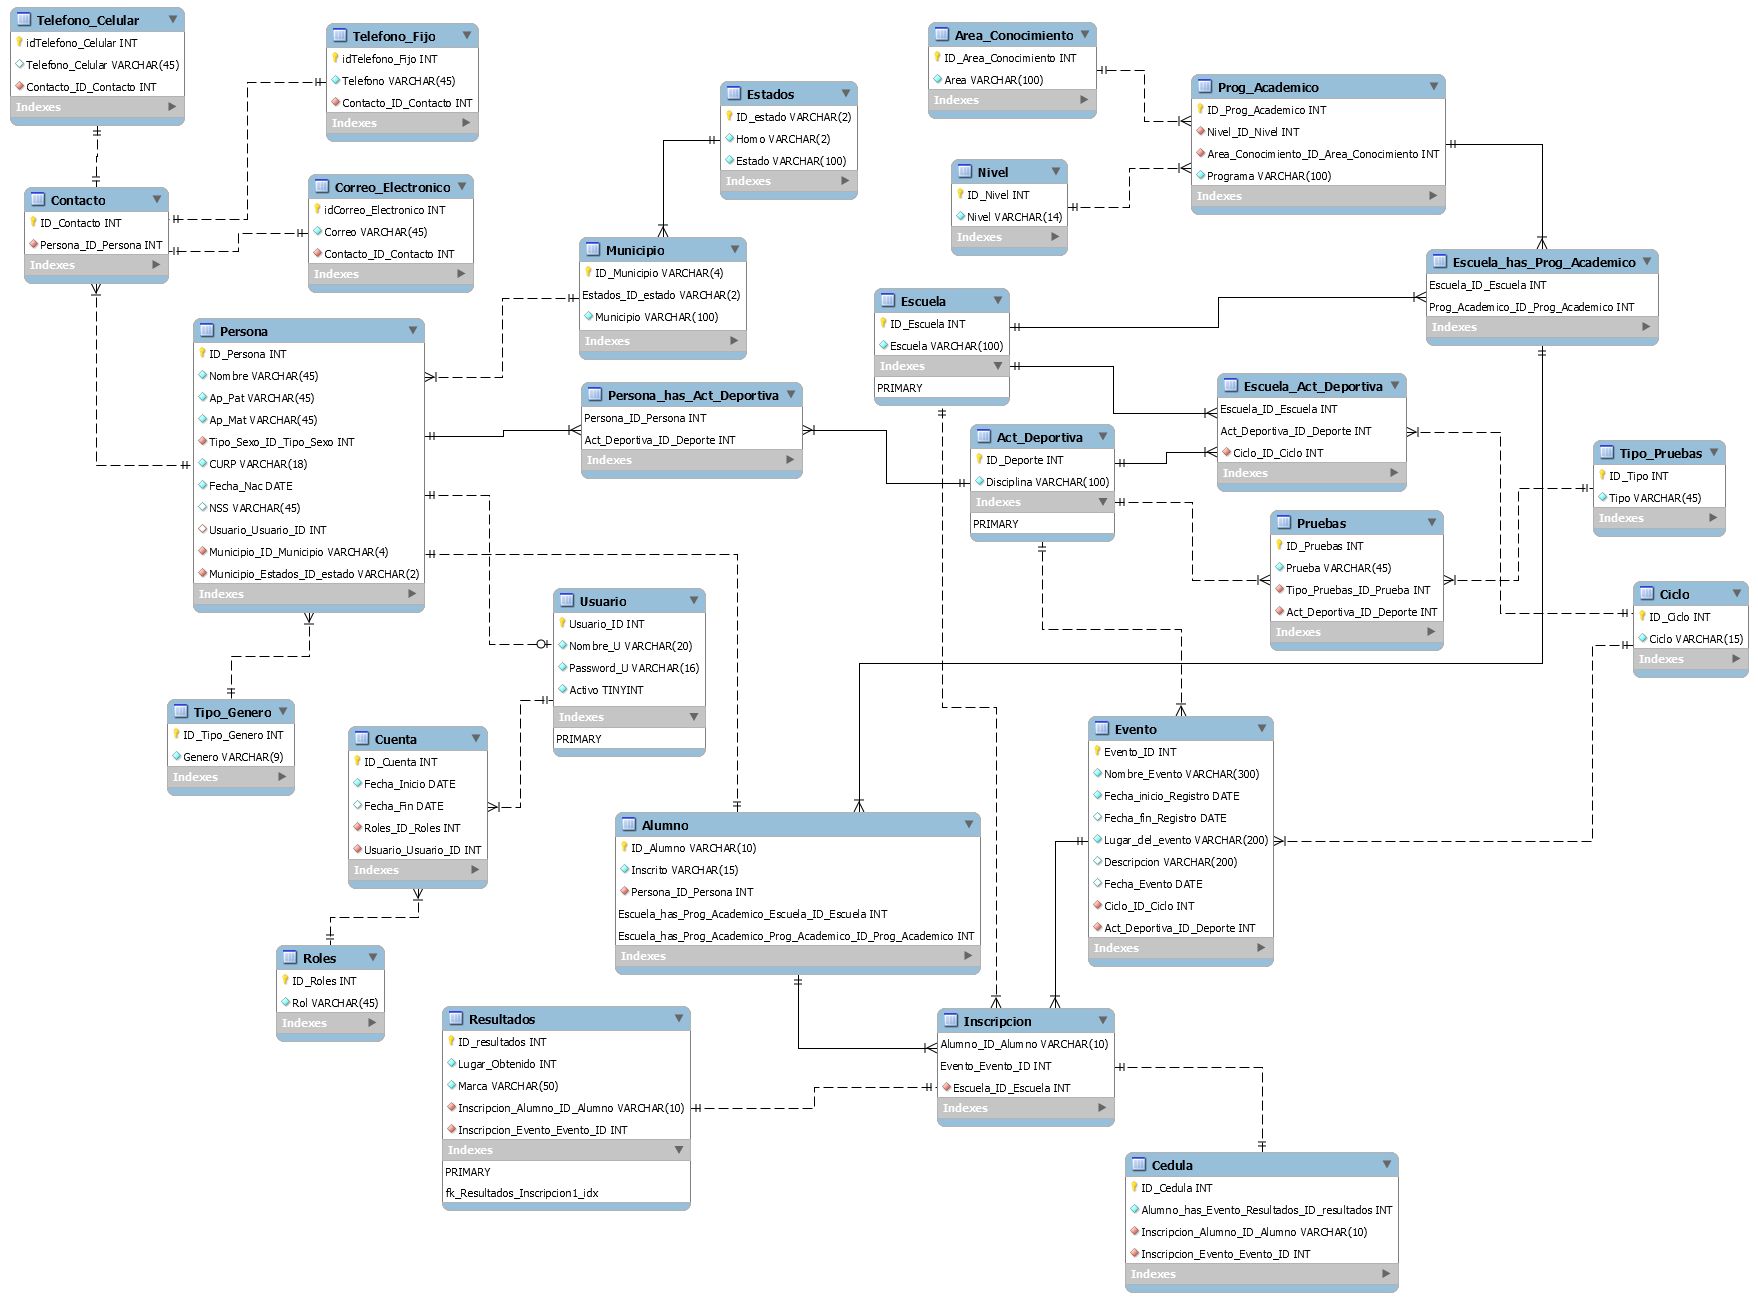
\includegraphics[angle=90, width=14cm, height=19cm]{Imagenes/bdrid.png}
			\caption{Estructura de la Base de Datos de RIDESCOM}
			\label{BaseDatos}
		\end{figure}
		
		
	
	\pagebreak
	
	\section{Apartado F: Entrevista}
		\noindent Entrevista con responsable de las actividades del Departamento de Formación Deportiva
		Buenas tardes, agradecemos el tiempo que nos esta brindando para mostrarle nuestra propuesta de Trabajo Terminal con la cual se pretende ayudar en el proceso de inscripción para los alumnos.
		\label{Entrevista}
		\begin{enumerate}
			\item ¿Cuál es el proceso actual para la inscripción a un evento interpolitécnico?\\
			El alumno tiene que acudir al departamento de Actividades Deportivas de su unidad académica, informar que quiere participar en un evento inrtepolitécnico. Con esto el coordinador procede a solicitar una identificación o documento probatorio que compruebe el estatus académico del alumno, a la vez el coordinador le proporciona una cédula de inscripción para que sea llenada y entrada. Si esto cumple puede continuar con su proceso en caso contrario se detiene el trámite. En cualquiera de los dos caso el alumno es informado del resultado final.
			
			\item ¿Hay límite de edad para los participantes?
			\item ¿Se tiene un formato definido para la inscripción?
			\item ¿Es necesario la comprobación de inscripción de los alumnos?
			\item ¿Cuántos deportes hay actualmente practicándose en el IPN?
			\item ¿Se cuenta con algún método de verificación de datos?
			\item Una vez concluido los eventos, ¿Qué sigue?
			\item ¿Cuánto tiempo suele tardarse en la publicación de los resultados?
			\item ¿Qué puntos se consideran en la generación de estadísticas?
		\end{enumerate} 
